% ICASSP-style final project report
% Project: Autoregressive Speech Prediction
% Author: Yang Jiekang, Student ID: 225010280
% Course: MDS5122

\documentclass{article}
\usepackage{spconf,amsmath,graphicx,hyperref}
\usepackage{booktabs}
\usepackage{multirow}
\usepackage{array}
\usepackage{url}

\graphicspath{{outputs/}}

\def\x{{\mathbf x}}
\def\L{{\cal L}}

\title{Autoregressive Speech Prediction with EnCodec and FACodec Token Language Models}

\name{Yang Jiekang}
\address{
	Student ID: 225010280 \\
	School of Science and Engineering \\
	Computer and Information Engineering \\
	The Chinese University of Hong Kong, Shenzhen \\
	Course: MDS5122
}

\begin{document}
	\ninept
	
	\maketitle
	
	\begin{abstract}
		This project implements an autoregressive speech prediction system based on discrete neural codec tokens. Given a 2-second speech context, the system predicts the following 1-second future speech segment. The main pipeline encodes waveforms into EnCodec tokens, trains a causal Transformer language model for next-token prediction, generates future tokens autoregressively, and decodes them back into waveforms. Experiments on WSJCAM0-style speech data show that the EnCodec small model improves over a copy baseline in reference-based metrics, achieving 0.351 STOI, 1.108 PESQ, and 1.485 DNSMOS on 644 test utterances. EnCodec oracle reconstruction provides a much higher upper bound of 0.910 STOI and 2.506 PESQ, indicating that the main bottleneck is future token prediction rather than codec reconstruction alone. I also compare EnCodec and FACodec oracle reconstruction and train six per-codebook FACodec Transformer language models. Compared with the full codec prediction framework in prior work, this project is a lightweight reproduction and extension that highlights the importance of multi-codebook modeling.
	\end{abstract}
	
	\begin{keywords}
		speech prediction, neural audio codec, EnCodec, FACodec, Transformer language model
	\end{keywords}
	
	\section{Introduction}
	\label{sec:intro}
	
	Autoregressive speech prediction aims to generate future speech from a given speech context. This task is similar to language modeling: instead of predicting future words from previous words, the model predicts future speech tokens from previous speech tokens. Neural audio codecs make this formulation practical because they convert continuous waveforms into discrete token sequences.
	
	In this project, I implement a codec-based autoregressive speech prediction system. The system first tokenizes speech using EnCodec, then trains a Transformer language model to predict future discrete tokens, and finally decodes the predicted tokens into waveforms. The main prediction task uses the first 2 seconds of an utterance as context and predicts the following 1 second. Objective scores are computed only on the predicted future segment.
	
	The project contains three main parts. First, I build and evaluate an EnCodec-based speech prediction pipeline with copy baseline, oracle reconstruction, greedy generation, and top-k sampling comparison. Second, I compare EnCodec and FACodec oracle reconstruction on a 16-utterance subset. Third, I train six separate FACodec Transformer language models, one for each FACodec codebook, and analyze the difficulty of modeling different codebooks.
	
	The main contribution is a complete reproducible implementation of codec-token-based speech prediction and a careful analysis of both EnCodec prediction performance and FACodec codebook predictability.
	
	\section{Related Work}
	\label{sec:related}
	
	Codec-based speech prediction has recently been studied by Wang et al. \cite{wang2026speech}, who proposed a system that encodes speech into codec tokens, predicts future tokens using a Transformer decoder, and reconstructs speech using the codec decoder. This project follows the same general idea, but implements a simplified system with explicit baselines and additional FACodec analysis.
	
	EnCodec \cite{defossez2023encodec} is a high-fidelity neural audio codec based on residual vector quantization. It encodes waveform signals into multiple streams of discrete codebook indices. Because these indices are discrete, they can be modeled using language modeling techniques.
	
	FACodec was introduced in NaturalSpeech 3 \cite{ju2024naturalspeech3}. It factorizes speech representations into multiple specialized codebooks, such as prosody, content, and residual-related components. Compared with EnCodec, FACodec may provide more structured token streams, but its multi-codebook nature also introduces additional modeling complexity.
	
	Transformer language models \cite{vaswani2017attention} are effective for autoregressive sequence modeling. Given a token sequence, a causal Transformer predicts each next token conditioned only on previous tokens. This makes it suitable for codec token prediction.
	
	\section{Method}
	\label{sec:method}
	
	\subsection{Problem formulation}
	
	Given an input speech waveform, the goal is to predict a future waveform segment from a previous context segment. In my experiments, each utterance is divided into a 2-second context and a 1-second future target. The model uses the 0s--2s context to predict the 2s--3s future segment.
	
	The codec-based pipeline contains three stages:
	
	\begin{enumerate}
		\item Encode waveform into discrete codec tokens.
		\item Predict future tokens using an autoregressive Transformer LM.
		\item Decode predicted tokens into a future waveform.
	\end{enumerate}
	
	The Transformer is trained with next-token cross-entropy loss:
	
	$$
	\mathcal{L} = - \sum_t \log p(x_t \mid x_{<t})
	$$
	
	where the token at time step t is predicted from its previous tokens.
	
	\subsection{EnCodec token modeling}
	
	For the main experiments, I use the EnCodec 24 kHz mono model with 6.0 kbps bandwidth. EnCodec produces 8 codebooks, each with a vocabulary size of 1024. A typical token tensor has shape such as 8 by 416.
	
	To reduce complexity, the current EnCodec language model predicts only the first EnCodec codebook. This is a lightweight design, but EnCodec decoding still requires all codebooks. Therefore, during waveform generation, the predicted first-codebook future tokens are combined with heuristic filling for the remaining codebooks. The main system uses a repeat-last strategy, where the last context token of each non-predicted codebook is repeated over the future duration.
	
	The main EnCodec small model uses greedy decoding. Although the generation metadata records temperature, top-k, and top-p values, the field \texttt{greedy=true} indicates that sampling is disabled for the main system.
	
	\subsection{Transformer LM architecture}
	
	The EnCodec small Transformer LM is a decoder-only causal Transformer. It contains token embeddings, positional embeddings, causal self-attention layers, feed-forward layers, layer normalization, and an output vocabulary projection.
	
	The model predicts first-codebook EnCodec tokens using next-token prediction. The main configuration is shown in Table \ref{tab:encodec_config}.
	
	\begin{table}[t]
		\centering
		\caption{Configuration of the EnCodec small Transformer LM.}
		\label{tab:encodec_config}
		\small
		\begin{tabular}{lc}
			\toprule
			\textbf{Parameter} & \textbf{Value} \\
			\midrule
			Vocabulary size & 1024 \\
			Sequence length & 512 \\
			Batch size & 8 \\
			Epochs & 20 \\
			Hidden dimension & 256 \\
			Transformer layers & 4 \\
			Attention heads & 4 \\
			FFN dimension & 1024 \\
			Learning rate & 0.0003 \\
			Parameters & 3.81M \\
			Best epoch & 18 \\
			Best valid loss & 2.4869 \\
			Best valid PPL & 12.0237 \\
			\bottomrule
		\end{tabular}
	\end{table}
	
	\subsection{FACodec per-codebook modeling}
	
	FACodec produces 6 discrete codebook streams. I train one Transformer LM independently for each codebook. The factorized modeling assumption is:
	
	$$
	p(\mathbf{x}) \approx \prod_{k=1}^{K} p(x_t^{(k)} \mid x_{<t}^{(k)})
	$$
	
	where K is the number of FACodec codebooks. In this project, K equals 6. Each FACodec codebook model uses vocabulary size 1024, sequence length 512, batch size 16, 20 epochs, hidden dimension 256, 4 layers, 4 heads, FFN dimension 1024, and learning rate 0.0003.
	
	This per-codebook design makes training simple and interpretable. It also allows direct comparison of modeling difficulty across FACodec codebooks.
	
	\section{Experiments}
	\label{sec:experiments}
	
	\subsection{Dataset and evaluation setup}
	
	The main EnCodec experiments use WSJCAM0-style speech data. The dataset contains 12,479 training utterances, 1,176 validation utterances, and 644 test utterances. EnCodec token extraction is performed using the 24 kHz model at 6.0 kbps.
	
	For future speech generation, the first 2 seconds of each utterance are used as context, and the model predicts the following 1 second. Evaluation compares only the predicted 2s--3s segment with the reference 2s--3s segment.
	
	I use STOI \cite{taal2011stoi}, PESQ \cite{rix2001pesq}, and DNSMOS \cite{reddy2022dnsmos} as objective evaluation metrics. STOI and PESQ are reference-based metrics and are computed between the predicted 2s--3s waveform and the ground-truth 2s--3s waveform after resampling both signals to 16 kHz. DNSMOS is a non-intrusive no-reference speech quality metric and is computed using the TorchMetrics implementation of DNSMOS P.835. Since each predicted future segment is only 1 second long, each predicted clip is repeated to satisfy the minimum DNSMOS inference window. I report the DNSMOS OVRL score as the final DNSMOS value.
	
	\subsection{Systems compared}
	
	I compare the following systems:
	
	\begin{itemize}
		\item \textbf{Copy baseline}: copies the 1s--2s context segment as the prediction for 2s--3s.
		\item \textbf{EnCodec oracle}: encodes and decodes the ground-truth waveform and evaluates reconstructed future speech.
		\item \textbf{EnCodec small}: predicts future first-codebook tokens using the trained Transformer LM with greedy decoding and repeat-last filling.
		\item \textbf{EnCodec top-k20}: uses top-k sampling with top-k equal to 20 and temperature 0.8 for comparison.
		\item \textbf{FACodec oracle small16}: evaluates FACodec reconstruction on 16 utterances.
	\end{itemize}
	
	\subsection{Full-set EnCodec prediction results}
	
	Table \ref{tab:full_results} reports the full-set prediction results on 644 test utterances. Higher values are better for STOI, PESQ, and DNSMOS. DNSMOS reports the OVRL score.
	
	\begin{table}[t]
		\centering
		\caption{Full-set evaluation results. Higher STOI, PESQ, and DNSMOS are better. DNSMOS reports the OVRL score.}
		\label{tab:full_results}
		\small
		\begin{tabular}{lcccc}
			\toprule
			\textbf{System} & \textbf{\# Utt.} & \textbf{STOI} & \textbf{PESQ} & \textbf{DNSMOS} \\
			\midrule
			Copy baseline & 644 & 0.137 & 1.053 & 2.480 \\
			EnCodec oracle & 644 & 0.910 & 2.506 & 2.071 \\
			EnCodec small & 644 & 0.351 & 1.108 & 1.485 \\
			EnCodec top-k20 & 644 & 0.204 & 1.086 & 1.618 \\
			\bottomrule
		\end{tabular}
	\end{table}
	
	The EnCodec small model reaches 0.351 STOI, 1.108 PESQ, and 1.485 DNSMOS. Compared with the copy baseline, it substantially improves STOI from 0.137 to 0.351. This suggests that the Transformer-predicted codec tokens are more consistent with the reference future speech than simply copying the previous context.
	
	However, the gap between EnCodec small and EnCodec oracle remains large. The oracle obtains 0.910 STOI and 2.506 PESQ, while EnCodec small obtains only 0.351 STOI and 1.108 PESQ. This suggests that the main bottleneck is not codec reconstruction alone, but accurate future token prediction.
	
	The copy baseline obtains the highest DNSMOS score, reaching 2.480. This does not mean that it is the best future prediction system. DNSMOS is a no-reference perceptual quality metric, so it evaluates whether the audio sounds natural and speech-like, but it does not compare the generated waveform with the true future segment. Since the copy baseline directly reuses a real speech waveform from the previous context, it can sound natural even though it does not match the actual future speech.
	
	Top-k20 sampling performs worse than the main greedy system in reference-based metrics. Its STOI decreases from 0.351 to 0.204, and PESQ decreases from 1.108 to 1.086. Although top-k20 obtains a slightly higher DNSMOS score than EnCodec small, this should be interpreted carefully because DNSMOS does not use the reference future signal. For this task, STOI and PESQ better reflect future prediction accuracy.
	
	\subsection{Oracle codec reconstruction}
	
	Table \ref{tab:oracle} compares EnCodec and FACodec oracle reconstruction on a 16-utterance subset. In this setting, the codec receives the ground-truth waveform, encodes it, and decodes it back to waveform. Therefore, the experiment evaluates codec reconstruction quality rather than future prediction quality.
	
	\begin{table}[t]
		\centering
		\caption{Oracle reconstruction comparison on 16 utterances.}
		\label{tab:oracle}
		\small
		\begin{tabular}{lcccc}
			\toprule
			\textbf{Codec} & \textbf{MSE} & \textbf{SNR} & \textbf{SI-SDR} & \textbf{Time} \\
			& & \textbf{dB} & \textbf{dB} & \textbf{s/item} \\
			\midrule
			EnCodec & 8.44e-5 & 3.618 & 2.072 & 0.111 \\
			FACodec & 1.03e-4 & 2.514 & -0.197 & 0.329 \\
			\bottomrule
		\end{tabular}
	\end{table}
	
	EnCodec gives better waveform-level reconstruction than FACodec on this subset. It has lower MSE, higher SNR, higher SI-SDR, and faster inference. FACodec is approximately 2.96 times slower in this experiment. However, FACodec still provides a useful structured representation with 6 factorized codebooks, which may be beneficial for future generative modeling.
	
	\subsection{FACodec codebook LM results}
	
	Table \ref{tab:facodec_lm} summarizes the FACodec per-codebook LM training results. All six codebook models were trained for 20 epochs.
	
	\begin{table}[t]
		\centering
		\caption{FACodec per-codebook Transformer LM results.}
		\label{tab:facodec_lm}
		\small
		\begin{tabular}{ccccc}
			\toprule
			\textbf{CB} & \textbf{Best Ep.} & \textbf{Best Loss} & \textbf{Best PPL} & \textbf{Final Loss} \\
			\midrule
			0 & 19 & 3.954 & 52.13 & 3.956 \\
			1 & 20 & 2.809 & 16.59 & 2.809 \\
			2 & 16 & 4.948 & 140.88 & 4.948 \\
			3 & 14 & 5.664 & 288.25 & 5.675 \\
			4 & 14 & 5.754 & 315.60 & 5.772 \\
			5 & 13 & 5.567 & 261.53 & 5.589 \\
			\bottomrule
		\end{tabular}
	\end{table}
	
	The results reveal a clear codebook-level difference. Codebook 1 is the easiest to model, with the lowest validation loss and perplexity. Codebook 0 is also relatively predictable. In contrast, codebooks 3, 4, and 5 have much higher perplexities. This suggests that later FACodec codebooks contain higher-entropy residual or fine acoustic information.
	
	\begin{figure}[t]
		\centering
		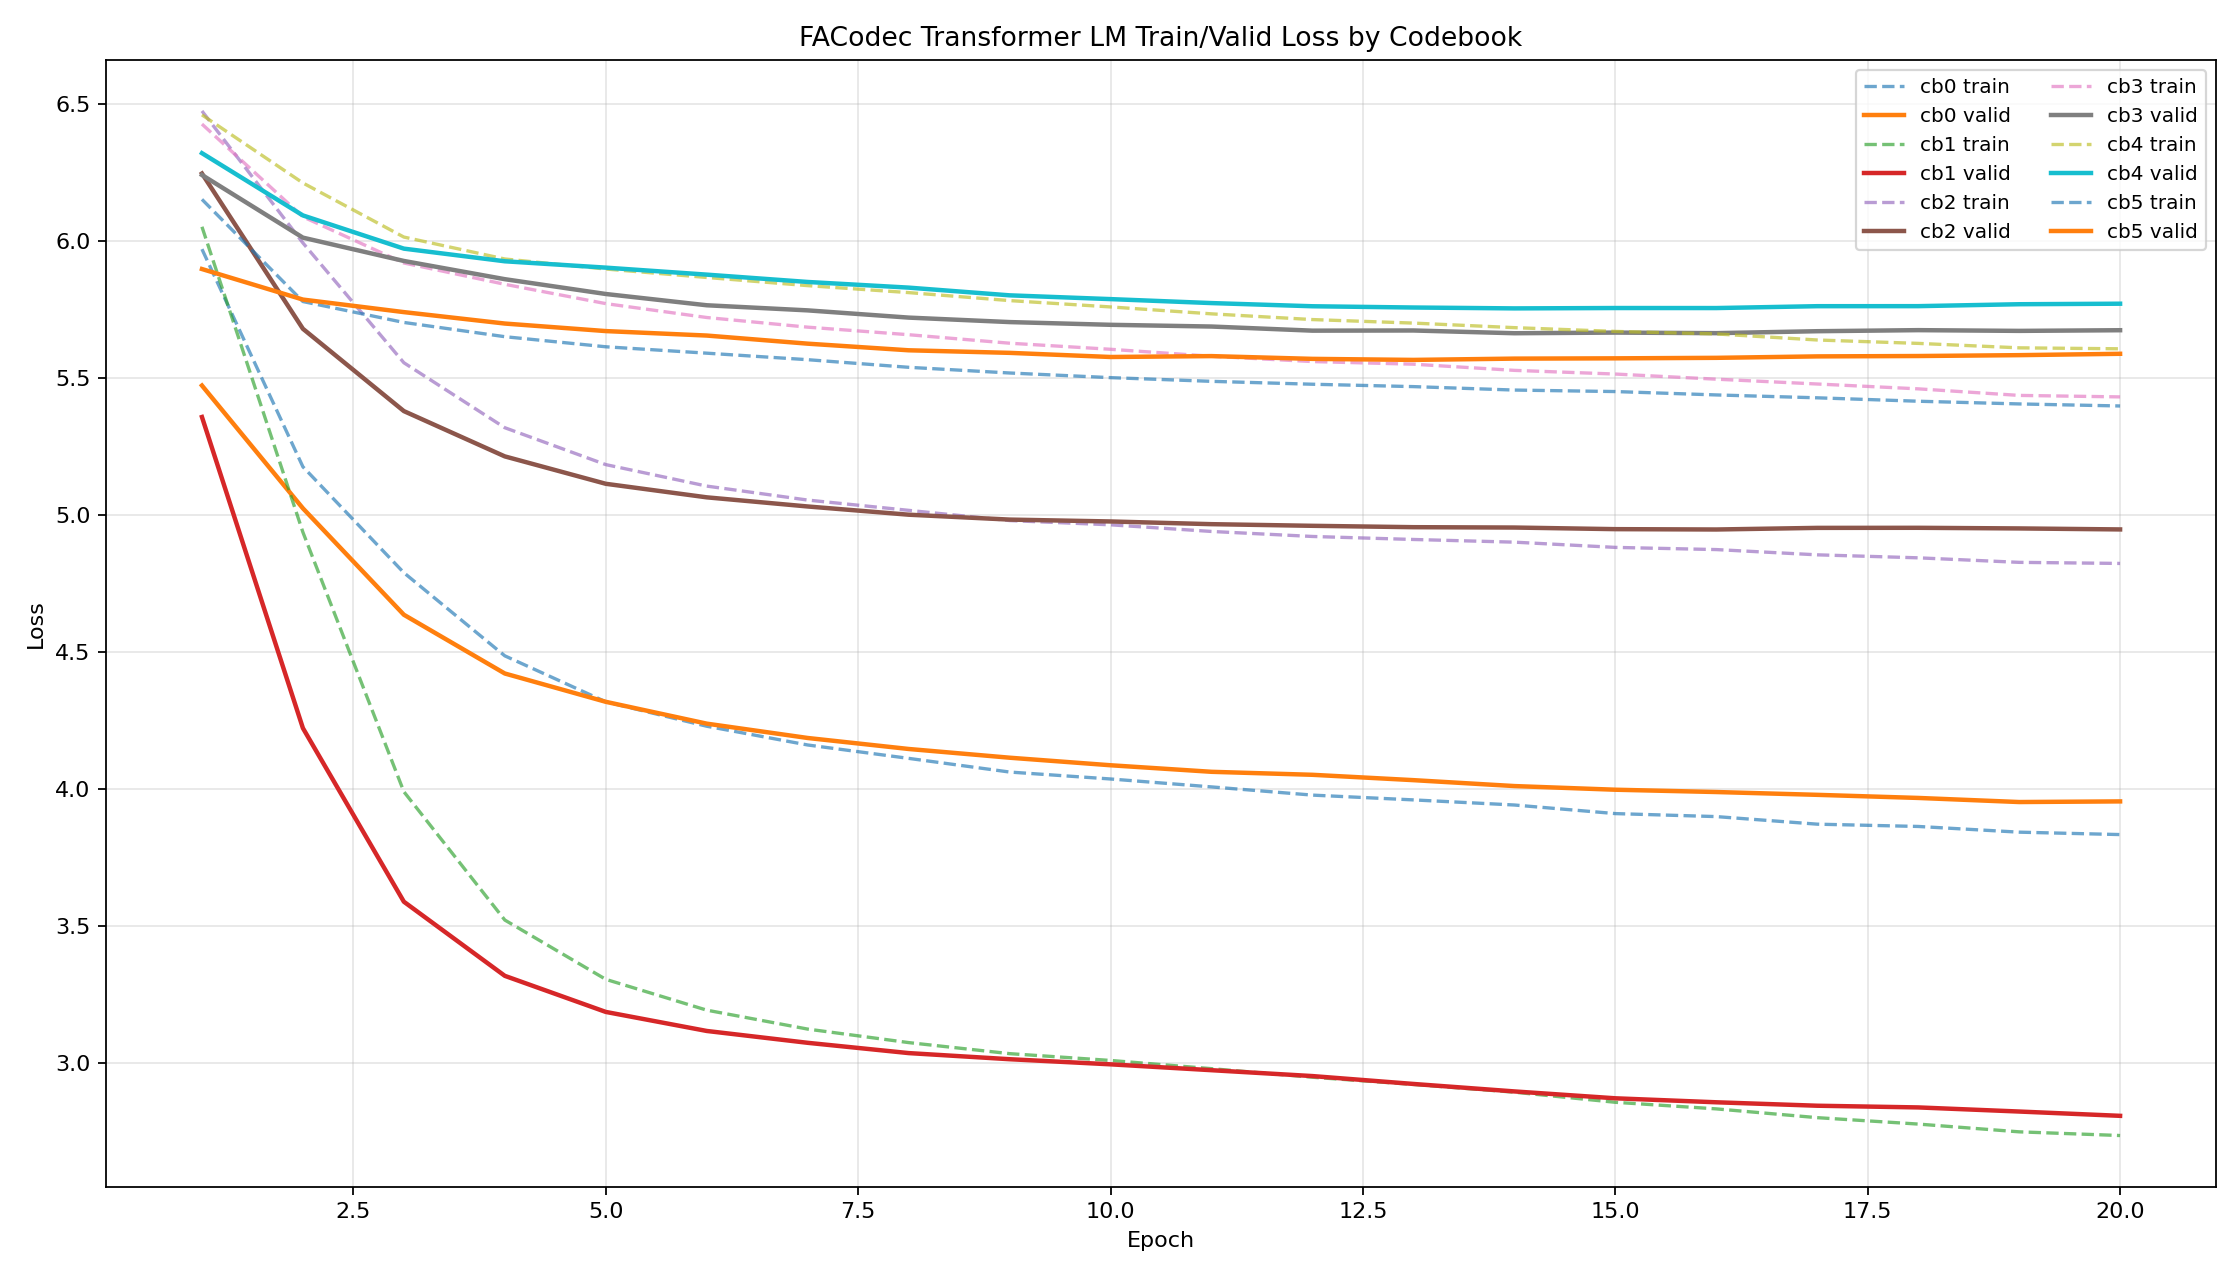
\includegraphics[width=\linewidth]{facodec_lm_loss_curves.png}
		\caption{Training and validation loss curves for FACodec per-codebook Transformer LMs.}
		\label{fig:facodec_curves}
	\end{figure}
	
	\begin{figure}[t]
		\centering
		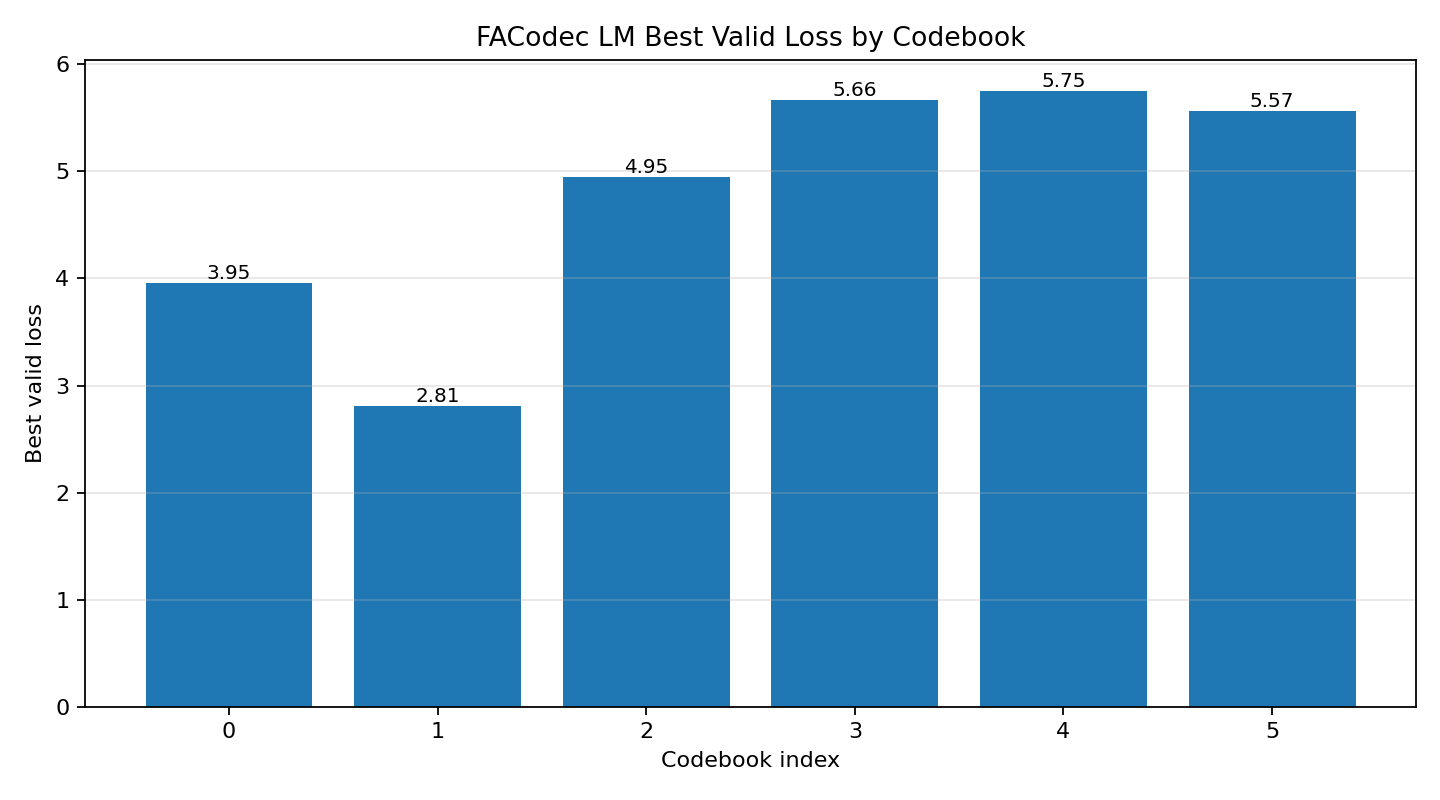
\includegraphics[width=\linewidth]{facodec_lm_best_valid_loss_bar.png}
		\caption{Best validation loss for each FACodec codebook. Later codebooks are harder to predict.}
		\label{fig:facodec_bar}
	\end{figure}
	
	\subsection{Larger EnCodec medium model}
	
	A larger EnCodec medium Transformer LM was also trained on Kaggle using a 644-utterance subset, with 580 utterances for training and 64 for validation. The model has 6 layers, 6 heads, hidden dimension 384, FFN dimension 1536, sequence length 768, batch size 8, and 11.73M parameters. It achieved a best validation loss of 2.158 and a best validation perplexity of 8.654 at epoch 15.
	
	However, full waveform-level generation and STOI, PESQ, and DNSMOS evaluation were not completed for the EnCodec medium checkpoint. Therefore, it is reported as a training extension rather than a directly comparable final prediction system.
	
	\section{Discussion}
	\label{sec:discussion}
	
	The experiments show that codec token modeling is a feasible approach for autoregressive speech prediction. The EnCodec small model clearly outperforms the copy baseline in reference-based prediction metrics, especially STOI. This means that the Transformer LM learns meaningful token transitions from speech context.
	
	At the same time, there is a large gap between EnCodec small and EnCodec oracle. The oracle obtains 0.910 STOI and 2.506 PESQ, while EnCodec small obtains 0.351 STOI and 1.108 PESQ. This gap shows that the codec itself is not the main limitation. The main challenge is predicting future tokens accurately.
	
	Compared with the speech prediction system in Wang et al. \cite{wang2026speech}, this project implements a simplified codec language modeling pipeline. The system in \cite{wang2026speech} studies a more complete codec-based prediction framework, while my final EnCodec system predicts only the first EnCodec codebook and fills the remaining codebooks with a repeat-last heuristic. Therefore, the results in this report should be interpreted as a lightweight reproduction and extension rather than a direct state-of-the-art reproduction. The large gap between EnCodec small and EnCodec oracle further confirms that more complete multi-codebook modeling, as motivated by \cite{wang2026speech}, is important for improving future speech prediction quality.
	
	The DNSMOS results reveal an important difference between acoustic naturalness and future prediction accuracy. The copy baseline receives the highest DNSMOS score because it copies a real speech segment and therefore produces natural-sounding audio. However, it performs poorly in STOI and PESQ because the copied segment does not match the true future speech. This shows that DNSMOS is useful for assessing perceptual speech quality, while STOI and PESQ are more directly tied to target-matching accuracy in this prediction task.
	
	One important limitation is that the current EnCodec LM predicts only the first codebook. The remaining codebooks are filled using repeat-last heuristics. Since non-first codebooks contain residual acoustic details, this approximation limits waveform quality and likely contributes to the relatively low DNSMOS of the learned prediction systems. A stronger system should model all EnCodec codebooks jointly or hierarchically.
	
	The FACodec experiments provide another useful insight. FACodec codebooks have very different predictability. Some codebooks are much easier to model, while later codebooks are much harder. This suggests that a future FACodec generation model should not treat all codebooks equally. A coarse-to-fine or conditional multi-codebook model may be more appropriate.
	
	\section{Conclusion}
	\label{sec:conclusion}
	
	This project implemented a codec-token-based autoregressive speech prediction system using EnCodec and FACodec. The main EnCodec small system predicts future first-codebook tokens from a 2-second context and decodes them into a 1-second future waveform. On 644 test utterances, it achieves 0.351 STOI, 1.108 PESQ, and 1.485 DNSMOS. It outperforms the copy baseline in reference-based prediction metrics but remains far below EnCodec oracle reconstruction.
	
	The FACodec experiments show that factorized codebooks have substantially different modeling difficulty. Codebook 1 is easiest to predict, while later codebooks have much higher perplexity. These results suggest that future work should focus on multi-codebook prediction, hierarchical token generation, and better decoding strategies that balance acoustic naturalness and reference consistency.
	
	Overall, the project demonstrates that discrete codec language modeling is a promising framework for speech prediction, while also highlighting the difficulty of long-horizon acoustic token generation. Compared with the full codec prediction direction in prior work, this implementation provides a compact and reproducible baseline that identifies future token prediction and multi-codebook generation as the main remaining challenges.
	
	\section{Acknowledgment}
	\label{sec:ack}
	
	The implementation and report writing process was assisted by online documentation and AI-based debugging tools. All experiments, analyses, and final interpretations were verified and organized by the author.
	
	\vfill\pagebreak
	
	\begin{thebibliography}{99}
		
		\bibitem{wang2026speech}
		H. Wang, Y. Yang, and D. L. Wang, ``A speech prediction model based on codec modeling and transformer decoding,'' \emph{Computer Speech and Language}, vol. 96, Article 101892, 2026.
		
		\bibitem{defossez2023encodec}
		A. D\'efossez, J. Copet, G. Synnaeve, and Y. Adi, ``High fidelity neural audio compression,'' \emph{Transactions on Machine Learning Research}, 2023.
		
		\bibitem{ju2024naturalspeech3}
		Z. Ju, Y. Wang, K. Shen, X. Tan, D. Xin, D. Yang, E. Liu, Y. Leng, K. Song, S. Tang, Z. Wu, T. Qin, X. Li, W. Ye, S. Zhang, J. Bian, L. He, J. Li, and S. Zhao, ``NaturalSpeech 3: Zero-shot speech synthesis with factorized codec and diffusion models,'' in \emph{Proc. ICML}, 2024, pp. 22605--22623.
		
		\bibitem{wsj0}
		J. Garofolo, D. Graff, D. Paul, and D. Pallett, ``CSR-I (WSJ0) Complete (LDC93S6A),'' Linguistic Data Consortium, Philadelphia, 1993.
		
		\bibitem{taal2011stoi}
		C. H. Taal, R. C. Hendriks, R. Heusdens, and J. Jensen, ``An algorithm for intelligibility prediction of time-frequency weighted noisy speech,'' \emph{IEEE Transactions on Audio, Speech, and Language Processing}, vol. 19, no. 7, pp. 2125--2136, 2011.
		
		\bibitem{rix2001pesq}
		A. W. Rix, J. G. Beerends, M. P. Hollier, and A. P. Hekstra, ``Perceptual evaluation of speech quality: A new method for speech quality assessment of telephone networks and codecs,'' in \emph{Proc. IEEE ICASSP}, 2001, pp. 749--752.
		
		\bibitem{reddy2022dnsmos}
		C. K. Reddy, V. Gopal, and R. Cutler, ``DNSMOS P.835: A non-intrusive perceptual objective speech quality metric to evaluate noise suppressors,'' in \emph{Proc. IEEE ICASSP}, 2022, pp. 886--890.
		
		\bibitem{vaswani2017attention}
		A. Vaswani, N. Shazeer, N. Parmar, J. Uszkoreit, L. Jones, A. N. Gomez, L. Kaiser, and I. Polosukhin, ``Attention is all you need,'' in \emph{Proc. NeurIPS}, 2017, pp. 5998--6008.
		
		\bibitem{yang2025robust}
		Y. Yang, H. Taherian, V. A. Kalkhorani, and D. L. Wang, ``Elevating robust ASR by decoupling multi-channel speaker separation and speech recognition,'' in \emph{Proc. ICASSP}, 2025.
		
	\end{thebibliography}
	
\end{document}
